\documentclass{article}
\usepackage{graphicx} % Required for inserting images
\usepackage{hyperref}
\usepackage{fancyvrb}
\usepackage[backend=biber, style=apa]{biblatex}
\addbibresource{references.bib}
\usepackage{setspace} % Add this to your preamble
\usepackage{wrapfig}


% Set smaller font size for all Verbatim environments
\fvset{
  fontsize=\small
}

\title{\huge Methodology for a Predictive Calculator\\
{\large Maturitätsarbeit, Kantonsschule Baden\\}
{\large Michael Schneider, Julia Smits}}
\author{Anton Mukin G4h}
\date{June 2025}

\setlength{\parindent}{0pt}

\begin{document}

\maketitle

\begin{figure}[htbp]
    \centering
    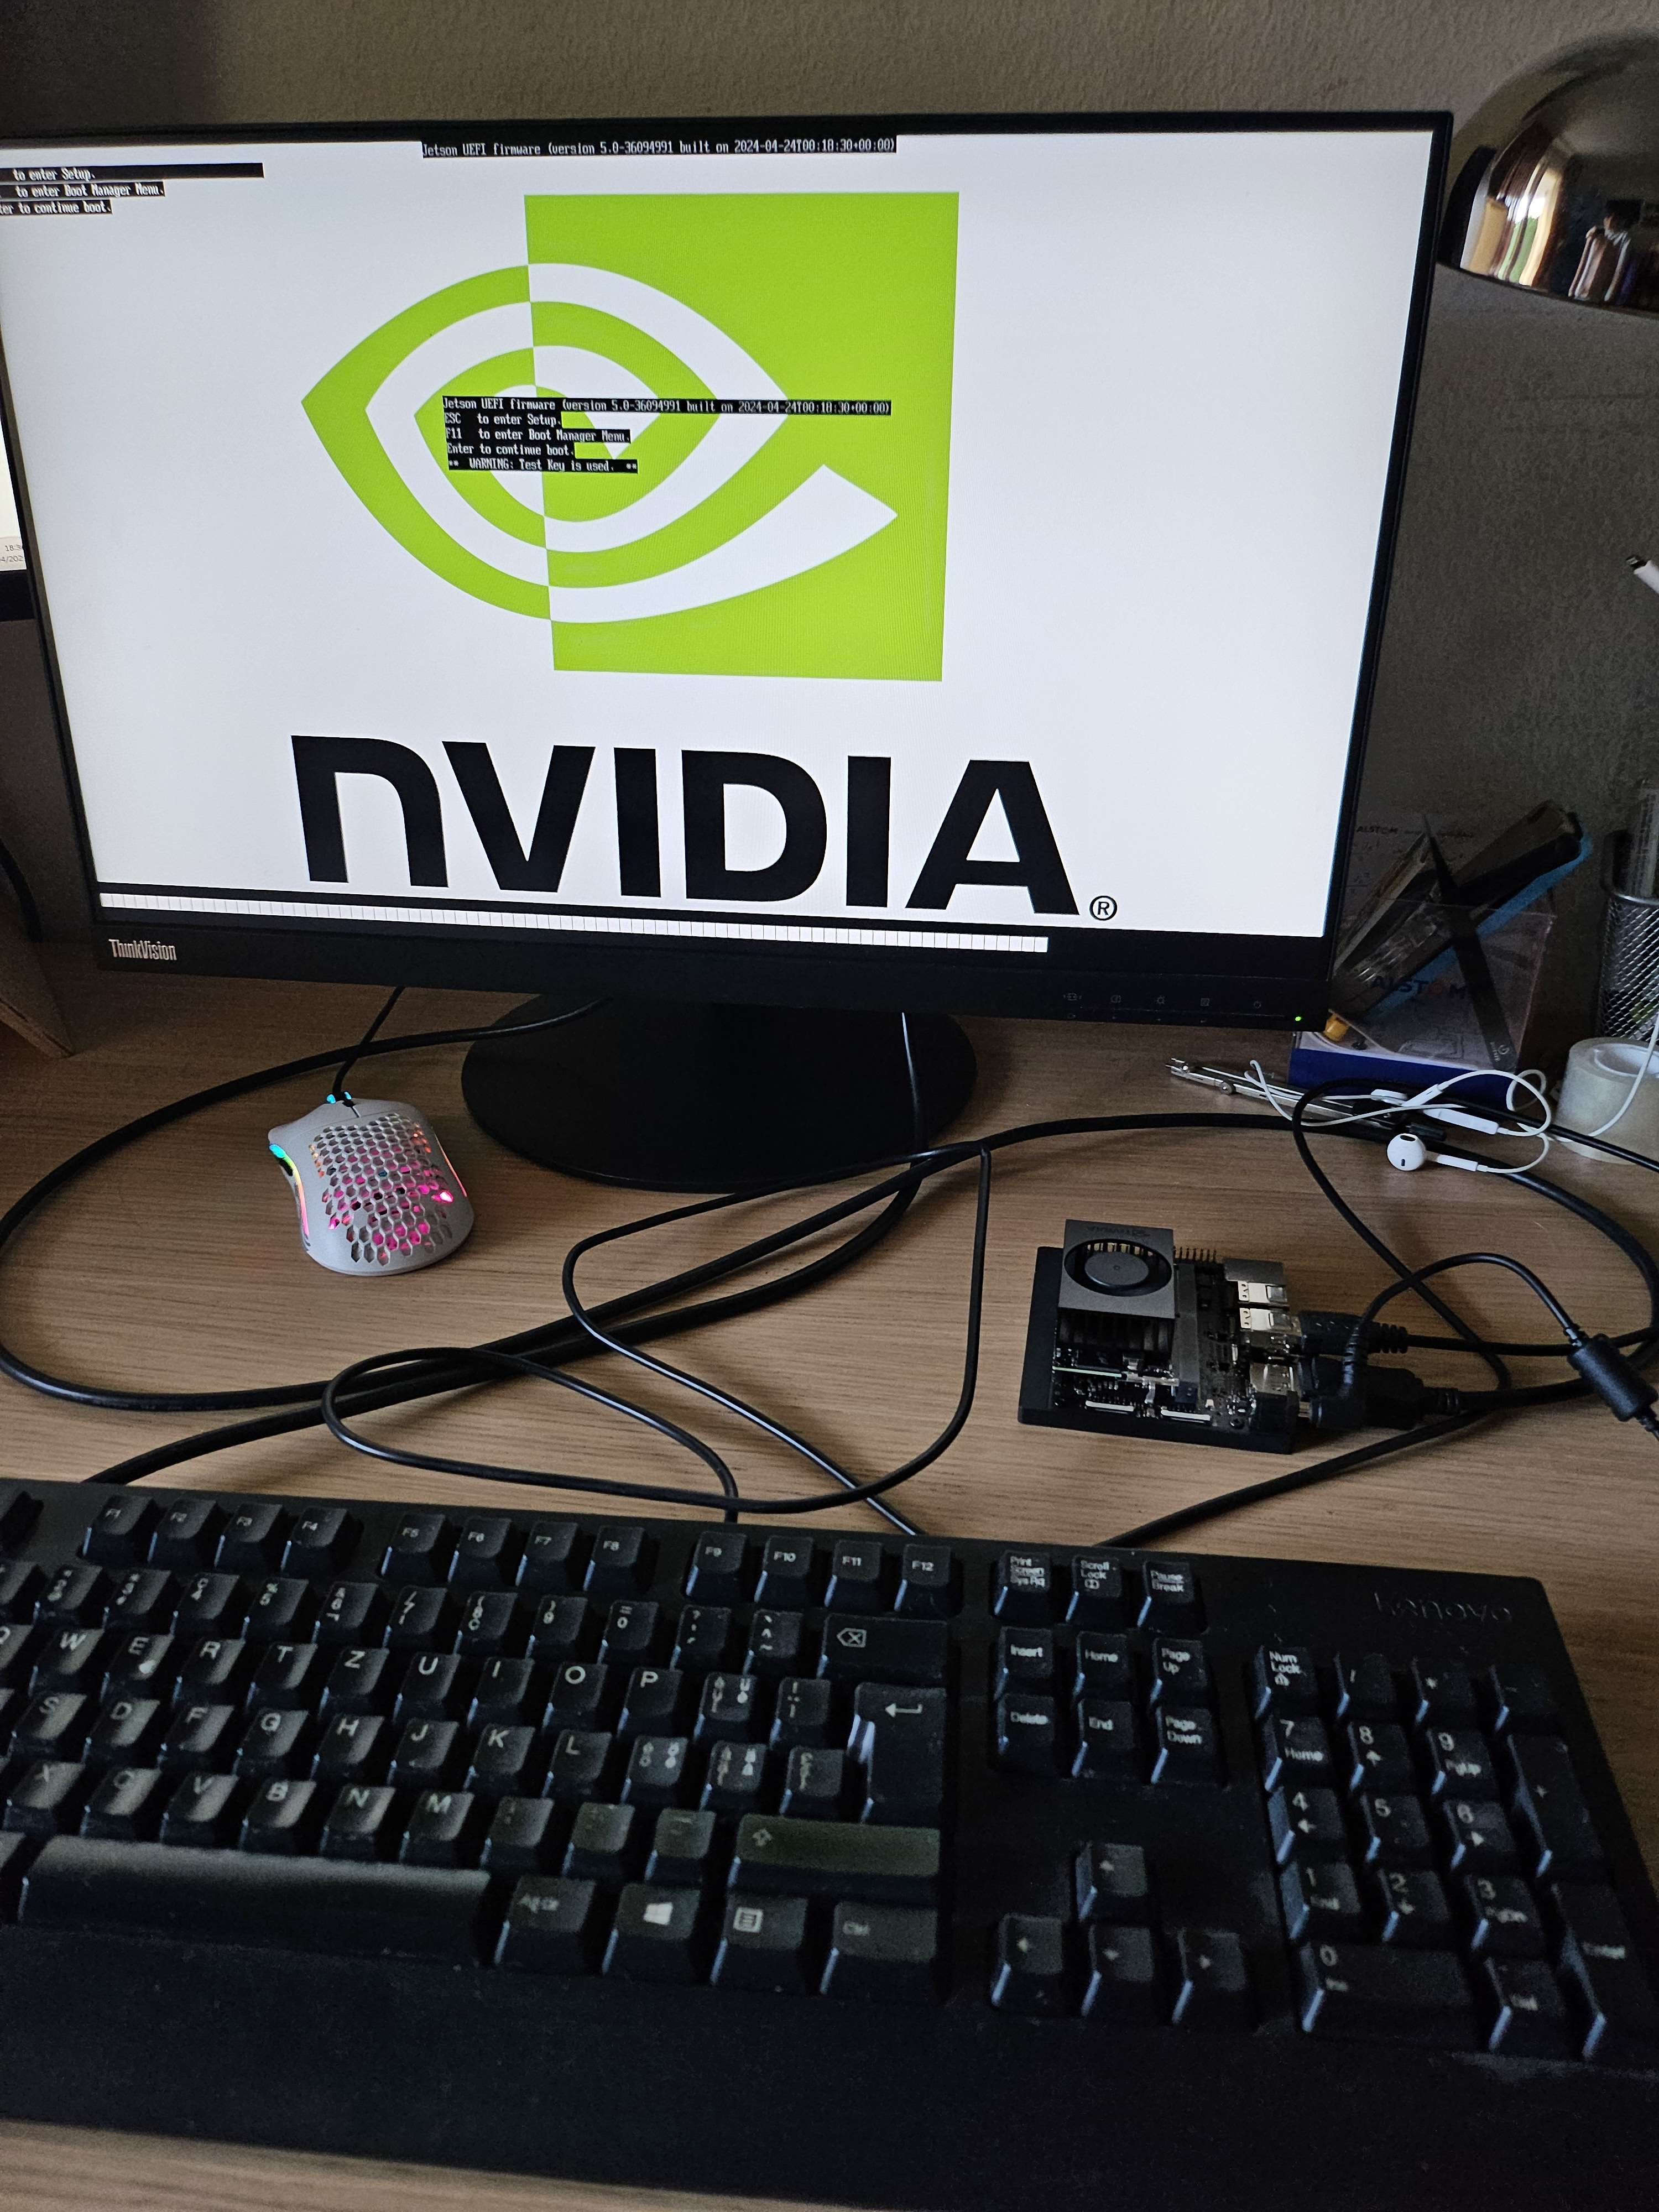
\includegraphics[width=0.7\textwidth]{images/JetsonBoot.jpg}
    \caption{Nvidia Jetson device during its boot sequence.}
    \label{fig:JetsonBoot}
\end{figure}

\newpage

\subsection{Brief Summary of the Project}
This Matura project investigates and evaluates the arithmetic capabilities of different neural networks.

The project began with a literature review to generate a hypothesis regarding the weaknesses of neural networks in performing simple arithmetic calculations. This literature review was submitted as the Zwischenprodukt, alongside a proof-of-concept notebook featuring a comparison of Feed-forward Neural Networks (FNNs) of different sizes.

The next step was to build a Recurrent Neural Network (RNN) and similar attention-based RNNs to investigate their arithmetic capabilities and compare them to those of the FNN using a benchmark.

The benchmark's baseline was defined as the performance of a basic FNN on different, but broadly similar, arithmetic tasks.

Afterwards, the same procedure was applied to the transformer type of neural network model. Here, their exact functionality was thoroughly investigated because of their unique architectures.

A similar workflow was repeated for larger, pre-trained models.

To sum things up, all findings were collected and evaluated comprehensively.


\subsection{Introduction to this document}
The goal of this document is to describe methodology applied in the current project, assist in reproducibility and to demonstrate how the findings discussed in the related document were obtained.

All of the code written for this project is available in the following GitHub repository:

\url{https://github.com/AntonStantan/matura}

\subsection{Software and Hardware specifications}

All code for this project is written in Python notebooks (Jupyter Lab). The preferred library used was \href{https://www.tensorflow.org/guide/keras}{tensorflow keras}.

Most of the models were trained locally on an Nvidia GPU device: \textit{Nvidia Jetson Orin Nano Super Developer Kit}, or alternatively on a Laptop: \textit{ThinkPad Z16 Gen 1} with a \textit{AMD Ryzen 7 PRO 6850H} CPU, which was used for calculations.





\newpage
\tableofcontents
\newpage

\section{Feed-forward Neural Networks (FNNs)}
For details on how an FNNs works, please refer to section 2 in \href{https://github.com/AntonStantan/matura/blob/main/zwischenProdukt/LiteraturstudieAnton.pdf}{the literature study}.

This section corresponds with the \href{https://github.com/AntonStantan/matura/tree/main/FNN}{/FNN directory} in the GitHub repository.

There are three notebooks here: \href{https://github.com/AntonStantan/matura/blob/main/FNN/FNN1.ipynb}{FNN1}, \href{https://github.com/AntonStantan/matura/blob/main/FNN/FNN2.ipynb}{FNN2} and \href{https://github.com/AntonStantan/matura/blob/main/FNN/FNN3.ipynb}{FNN3}.

\subsection{Train and Test data}
To define the training data, the decision was made to exclusively use subtraction and addition. The arithmetic expressions were defined to consist of two operators (+ or -) and three integers within the range $[-5, 5]$.

The reasons for these definitions are that + and - are the two simplest operators. The decision to introduce the model to three numbers, instead of the more common two, was made in the hope of simplifying the transition to more numbers in a later stage.

For example, the first three entries are:
\[
1 - -2 + 3 \qquad -2 + -3 - -5 \qquad 3 - 1 - 0
\]
{\small In total, there are 1907 such expressions in the training data.}
\\[2em]
The test data is also defined in a slightly unconventional manner. It is split into three categories.
\begin{itemize}
    \item Inside of the number range: Expressions identical in structure to the training data but not present in the training set.
    \item Outside of the number range: The same expression structures, but with numbers in the ranges $[-8, -5]$ and $[5, 8]$, e.g.,
\[
-6 + 6 + 8 \qquad -7 + 6 + 7 \qquad 5 - -6 - 6
\]
    \item Longer expressions: Expressions of different lengths. Specifically, there are between 2 and 8 numbers inside of the $[-5, 5]$ range, e.g.,
\[
-5 + 1 \qquad 3 + -1 + 4 + -2 + -4 \qquad -2 + 1 + 5 + -5 - -2 + -1 - 2 - 5
\]
\end{itemize}

\subsection{Tokenizer}

Because only tensors with floats can be passed into a model, the train and test data are always processed by a tokenizer before entering a neural network, as described by \cite{geeksforgeeks_nlp_tokenizing}.

Traditionally, a tokenizer assigns each prevalent character in the data a number, but because this project works with numerical data, this is not needed. Only the characters $+$ and $-$ need to be assigned a number.

For this project, the decision was made to work with: $1.0$ replacing $+$ and $0.0$ replacing $-$.
\\[1em]
Padding is also added, because a network trained on short expressions with only 3 numbers cannot process long expressions with more numbers (higher-dimensional vectors). Padding increases the length of those short expressions, by inflating them with values that dont represent any information.

To differentiate it from all other integers, a padding value of $0.5$ was defined.
\\[1em]
Consequently, an expression that was passed through the tokenizer and extended with padding would appear as follows:
$$
[1.\qquad 0.\qquad -2.\qquad 1.\qquad 3\quad 0.5\quad 0.5\quad 0.5\quad 0.5\quad 0.5\quad 0.5\quad 0.5\quad 0.5\quad 0.5\quad 0.5]
$$
\subsection{Training a Neural Network Using Tensorflow}
This subsection will show how the models used in this project were first defined and then trained with TensorFlow on the example of a simple FNN.
\\[2em]
To begin, the necessary libraries are imported.
\begin{Verbatim}
import tensorflow as tf
from tensorflow import keras
from tensorflow.keras.layers import Dense, Layer, Dropout
from tensorflow.keras import layers, Sequential
from tensorflow.keras.layers import PReLU
\end{Verbatim}

Next, a dataset is created from the train and validation data discussed in the previous subsection. Batches of 32 are used. The validation data is similar to the in-range test data, but with fewer expressions.
\begin{Verbatim}
batch_size = 32
train_dataset = tf.data.Dataset.from_tensor_slices((x_train, y_train))
.shuffle(len(x_train)).batch(batch_size)
val_dataset = tf.data.Dataset.from_tensor_slices((x_val, y_val))
.batch(batch_size)
\end{Verbatim}

The model can now be defined using tf.keras.Sequential. The model's architecture is clearly visible. In this example, the model has two dense layers with 64 neurons each.

The activation function used is PReLU, as this was the most promising in \cite{trask2018neuralarithmeticlogicunits}.

Dropout is included to prevent overfitting. In most models used in this project, it was not necessary.

As shown, the input shape must be defined when defining the model.

Additionally, it should be noted that the output layer only consists of a single neuron with a linear activation function. This means the model created is a regression model, which is similar to not having a decoder.

\newpage
\begin{Verbatim}
input_shape = (15,)
model = Sequential([
    keras.Input(shape = input_shape),     #input

    Dense(64),                            #first dense layer
    PReLU(),                              #PReLU activation function
    Dropout(0.1),                         #dropout layer

    Dense(64),                            #second dense layer
    PReLU(),                                
    Dropout(0.1),                           

    Dense(1, activation='linear')         #output layer
])
\end{Verbatim}

The next step is to compile the model by choosing an optimizer and a loss calculation, in this case, Mean Squared Error (MSE).
\begin{Verbatim}
model.compile(optimizer="adam", loss="mse")
\end{Verbatim}

The last remaining step is to fit the model on some data. The model will be fitted on the previously defined train and validation data. The training process will take 200 epochs to complete or might be aborted preemptively if the model starts to overfit and early stopping is triggered.

\begin{Verbatim}
model.fit(
    train_dataset,
    validation_data=val_dataset,
    epochs=200,
    callbacks=[early_stopping],
    verbose=1
)
\end{Verbatim}

\subsection{FNN1 and FNN2 Notebooks}
In FNN1, a simple FNN was created, its performance was evaluated, and FNNs of different sizes were compared against each other in a heatmap. It is noteworthy that the models here were used with a bootstrap, meaning multiple models with the same sizes were trained and then used to give one combined prediction. This was done to reduce noise. In later notebooks, this will not be the case, as this makes it more difficult to accurately evaluate a model.
\\[2em]
FNN2 includes a model with hyperparameters (in this case, the number of neurons, the number of layers, and whether or not to use dropout) chosen by the KerasTuner. This is, in simple terms, an automation process: it picks out models with different hyperparameters, trains them, and compares their performance on validation data. The model with the best-performing hyperparameters will be chosen as the best model.

The model in FNN2 is evaluated inside that notebook, and its benchmark is also calculated there.

\subsection{The Benchmark}
To calculate the benchmark, a model is evaluated on four categories: the test data inside the number range defined for training data, outside of the number range with numbers inside of the number range, longer expressions, and a relative MSE of the test data with numbers outside of the range.

Refer to the code below:
\begin{Verbatim}
benchmark = 0
benchmark += baseline_deviation / (meanDiff_InRange**2) / 4
benchmark += baseline_out_deviation / (meanDiff_OutRange**2) / 4
benchmark += baseline_long_deviation / (meanDiff_LongRange**2) / 4
benchmark += baseline_relError / (meanDiff_OutRelRange**2) / 4
print(f"Benchmark: {benchmark}")
\end{Verbatim}

The use of a relative error penalizes mistakes on "simpler" expressions and is less harsh on more "difficult" ones. Expressions whose absolute result is small are easier for a neural network to solve, while a larger absolute result is more difficult to calculate.

For the same reason, two more adjustments have been made: 

For longer expressions, only expressions with 4 numbers were used.

For expressions with numbers outside the range, the expression was only used if the absolute values of all three numbers added up to 22.

These subsets were chosen because of their reasonable MSE of around 10 each.
\\[1em]
This, as well as the inclusion of the relative MSE, is done in hopes of bringing the benchmarks of different models closer together and increasing the linearity between them. This makes the benchmark more tractable and consistent for comparison.

The baseline values are defined to be from an FNN model with 30 neurons and two dense layers. It is trained over a period of 200 epochs with early stopping enabled.

As is clearly observable in the code for calculating the benchmark, using this formula defines a model with the same performance as the baseline model to have a benchmark of 1. Models performing worse or better on the test data yield scores below or above 1, respectively.

\subsection{FNN3 with Positional Encoding}

In the notebook \href{https://github.com/AntonStantan/matura/blob/main/FNN/FNN3.ipynb}{FNN3}, a positional embedding layer is added to the model, and a Keras tuner tunes the hyperparameters of the model to an optimum. The formula used is the one from \cite{vaswani2023attentionneed}.


\section{Recurrent Neural Network (RNN)}

RNNs process sequential data by calculating a hidden state value, which is passed from one timestep to the next. For details on how RNNs work, refer to the corresponding section in \href{https://github.com/AntonStantan/matura/blob/main/documentation/findings/findings.pdf}{the findings document}.

\subsection{RNN0 and RNN2}
The \href{https://github.com/AntonStantan/matura/blob/main/RNN/RNN0.ipynb}{RNN0} notebook is a simplistic model with RNN architecture.

An RNN model consisting of 2 dense layers with 50 neurons each:

\begin{Verbatim}
model = keras.Sequential([
    keras.Input(shape=(input_shape, 1)),
    keras.layers.SimpleRNN(50, return_sequences=True),
    keras.layers.PReLU(),
    keras.layers.SimpleRNN(50),
    keras.layers.PReLU(),
    keras.layers.Dense(1, activation = "linear")
])
\end{Verbatim}
Note that `return\_sequences = True`. This is necessary for a subsequent layer. By default, this is set to false because RNNs are frequently used with just one layer for applications like Natural Language Processing (NLP) or time-series analysis, such as stock market prediction.

The same notebook used in FNN2 was adapted to work with RNNs in the notebook \href{https://github.com/AntonStantan/matura/blob/main/RNN/RNN2.ipynb}{RNN2}. As in FNN2, the KerasTuner was used for finding the optimal number of neurons and layers, as well as whether or not to include dropout after a dense layer.

Useful sources for the creation of the first RNN prototype:
\cite{bowman2015recursiveneuralnetworkslearn, tensorflow_keras_rnn, ibm_rnn}


\section{Attention and Transformers}

\subsection{Attentional RNNs}
For the sake of transitioning from RNNs to transformers, an attentional RNN model was trained and evaluated.

It consisted of a bidirectional\footnote{This means input is being processed from front to back and from back to front. It allows the LSTM to get a richer and broader context representation} Long Short-Term Memory (LSTM) layer, used as the encoder, and a self-attention mechanism for attention.

\begin{Verbatim}
#Encoder:
encoder_inputs = Input(shape = (len(x_train[0]), 1))
encoder_outputs = Bidirectional(LSTM(64, return_sequences=True))(encoder_inputs)

#self-attention mechanism
attention_outputs = Attention()([encoder_outputs, encoder_outputs])

#condensing into a single vector
context_vector = GlobalAveragePooling1D()(attention_outputs)

#output layer (Decoder)
output = Dense(1, activation = "linear")(context_vector)

model = Model(inputs = encoder_inputs, outputs = output)
\end{Verbatim}

This bidirectional LSTM with attention was realized in \href{https://github.com/AntonStantan/matura/blob/main/attentional-RNN/g4gLSTM.ipynb}{the g4gLSTM notebook}. It contains a model built with the help of code from \cite{geeksforgeeks_attention_bilstm}.

A number of 35 LSTM units were chosen for the encoder because of its previous performance (with bootstrapping), visible in \href{https://github.com/AntonStantan/matura/blob/main/attentional-RNN/previousHeatmap.png}{a heatmap}.
\\[2em]
In the directory \href{https://github.com/AntonStantan/matura/tree/main/RNN/Heatmaps}{/RNN/Heatmaps}, some heatmaps are presented; these were used to evaluate which model architecture to add attention to. Even though Gated Recurrent Units (GRUs) showed better results, they were not implemented because of the lack of online documentation for using attentional GRUs. This led to the choice of attentional LSTMs.

Nevertheless, the GRU architecture is still discussed in the findings document.

\newpage
\subsection{Transformers}

The original paper by \cite{vaswani2023attentionneed} was used as an example for building a replica model, which later was adjusted for better performance on the specific tasks in this project. The architectures used in this project resemble the one that first introduced the transformer architecture with one small difference: They are Regression models, not the sequence-to-sequence (seq2seq) type from the paper.



\begin{figure}[htbp]
    \centering
    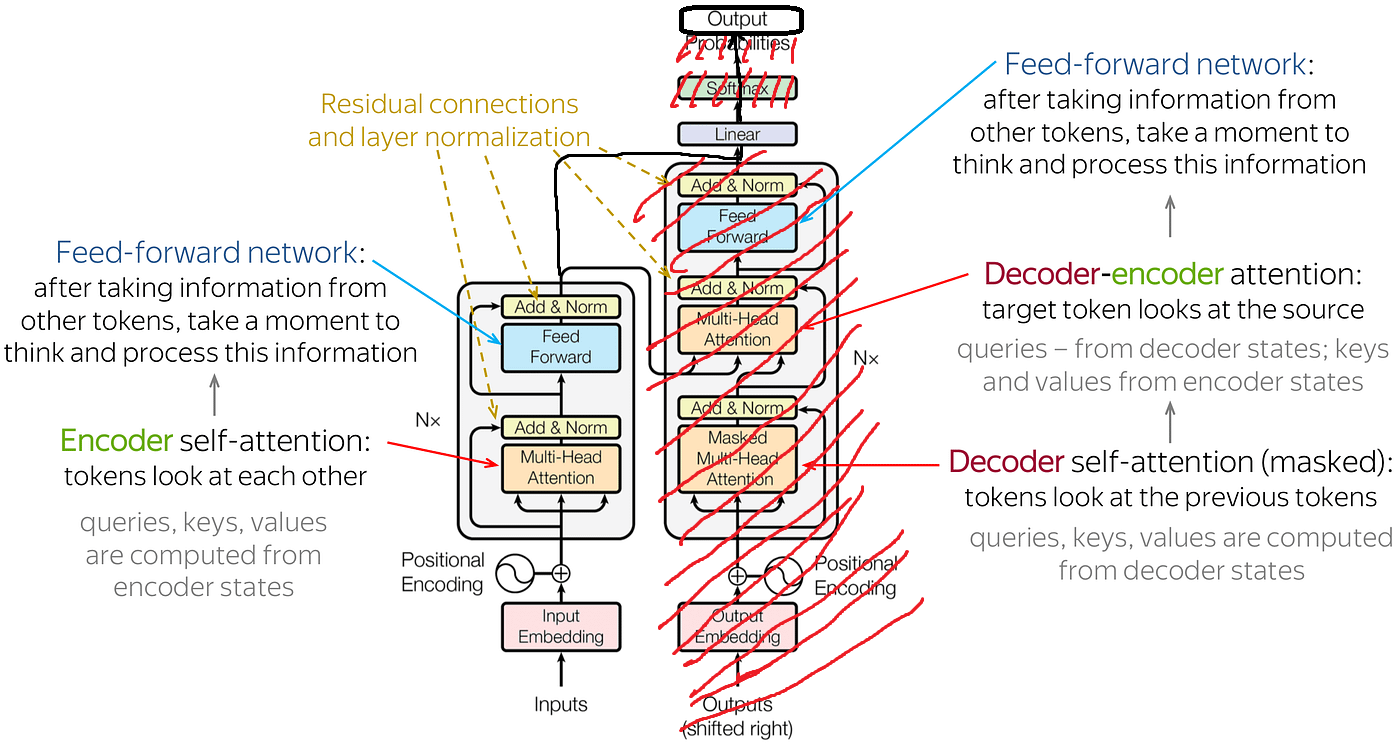
\includegraphics[width=0.5\paperwidth]{images/transformerSeq2Seq.png}
    \caption{A Seq2Seq model from \cite{vaswani2023attentionneed}. The 
    Encoder-only model used in this project is the same, except the decoder 
    part is skipped; in the image, this part has been crossed out with red. \href{https://www.cloud.studio/ai-llm-how-do-llms-work}{Source for figure}}
    \label{fig:transformerSeq2Seq}
\end{figure}

To code this in Python, an object-oriented approach has been taken, with classes consisting of other classes in a nested structure, similar to a matryoshka doll.

Below is the hierarchy:

\begin{itemize}
    \item Transformer which encapsulates embedding and positional encoding, as well as the encoder and a final one-neuron-FNN with a linear activation.
    \item Encoder containing encoding layers and dropout.
    \item Encoding layer consisting of the MHA and pointwise-FNN, as well as layer normalization and dropout (included in the original paper to prevent dropout)
    \item Multi-Head Attention (MHA) and pointwise-FNN
    \item Scaled Dot-Product (SDP) Attention
\end{itemize}

A model with the same hyperparameters as the ones used by \cite{vaswani2023attentionneed} can be found in \href{https://github.com/AntonStantan/matura/blob/main/transformer/transformer0.ipynb}{transformer0}.

Unfortunately, this model gets stuck in a local minimum during training, as can be seen at the bottom of its notebook. The minimum is simply predicting a number close to 0 for every expression.

This is an undesirable outcome, necessitating the tuning of the model's hyperparameters. This is done with the help of KerasTuner.

A couple of additional minor adjustments were made to the model before applying the KerasTuner, mainly switching to the AdamW optimizer, because it is better than Adam for transformers \cite{loshchilov2019decoupledweightdecayregularization}. A learning rate scheduler with warmup and cosine decay was also used. This means that, unlike before when the learning rate stayed constant throughout the training, the learning rate now changes. It is higher in the beginning and decays towards the end. This assists the model in taking larger optimization steps initially, thereby overcoming local minima, before proceeding with more precise, smaller steps towards the end of the training.

\begin{figure}[htbp]
    \centering
    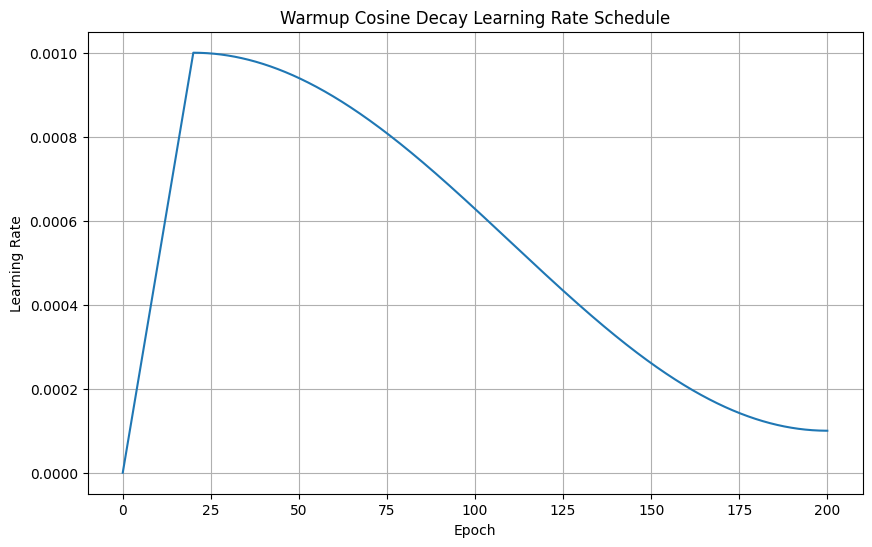
\includegraphics[width=0.5\paperwidth]{images/learningRate.png}
    \caption{This is how the learning rate could look for a model being trained over a period of 200 epochs when using a cosine decay with a linear warmup, as in this project. (Except for the changing peak learning rate, all other parameters are the same as the ones used in this project.)}
    \label{fig:learningrate}
\end{figure}

In contrast to the FNN or the RNN, a transformer has to be trained on other hyperparameters:
\begin{itemize}
    \item The number of heads inside the MHA
    \item The number of dimensions tensors have inside the model
    \item The number of encoding layers
    \item The number of neurons in the layer inside of the pointwise-FNN
    \item Whether to use dropout or not
    \item The peak learning rate after warmup and after the cosine decay
\end{itemize}


In the notebooks \href{https://github.com/AntonStantan/matura/blob/main/transformer/transformer4.ipynb}{transformer4} and \href{https://github.com/AntonStantan/matura/blob/main/transformer/transformer5.ipynb}{transformer5}, you can look at models with successfully tuned hyperparameters displaying promising performance on the benchmark.

The difference between them is that Transformer5 is a larger model than Transformer4.

\section{Pre-trained Transformers}

The final model type to be analyzed was fine-tuned pre-trained LLMs. Since working with them is completely different than working with locally trained neural networks, extensive research was required before commencing the work.
\\[1em]
Significant effort was dedicated to resolving library compatibility issues for the amd64 architecture system on the Jetson device. The final solution was using \href{https://github.com/dusty-nv/jetson-containers}{jetson-containers}, which offer a Docker container optimized for the Jetson system. Specifically, the container called `bitsandbytes` has most of the libraries needed for this project; the few remaining ones can be installed manually using: \texttt{pip install}.


\subsection{Gemini 2.5 Pro}
The first model to be fine-tuned was Gemini 2.5 Pro. This model was selected partly because of the author's familiarity with it and its high ranking in the \href{https://lmarena.ai/leaderboard}{LMArena}.
Fine-tuning had to be done on a remote server hosted by Google Cloud because of the model's size.

In the end, the costs for their service amounted to CHF 83.58.

The fine-tuning was done using VertexAI services. First, a .json file with the training data\footnote{For fine-tuning, the training set used was the combination of the training and validation data from before. This is because the VertexAI website had a tedious setup for validation data and this wouldn't have a big impact on results anyway.} had to be created and uploaded. Afterwards, the model was fine-tuned in the notebook \href{https://github.com/AntonStantan/matura/blob/main/pre-trained-tranformers/gemini_vertex.ipynb}{gemini\_vertex} using Vertex SDK. The resulting model is loaded into an endpoint on the Google Cloud servers.

To access the new, fine-tuned model and be able to evaluate it, a fairly simplistic notebook is created: \href{https://github.com/AntonStantan/matura/blob/main/pre-trained-tranformers/gemini_vertex_predict.ipynb}{gemini\_vertex\_predict}.

There, the model is loaded in from its endpoint and used to predict test data.

\subsection{Gemma 3}
For diversity, a small (Gemma3 1B parameters) and a tiny (Gemma3 270M parameters) model were chosen.

Because of their size, they can be fine-tuned locally on the Jetson device. They are fine-tuned with the SFTTrainer provided by `trl`.\footnote{We cannot use the standard Trainer from Hugging Face because the fine-tuning we do is supervised; hence the name: Supervised Fine-Tuning (SFT)} \href{https://huggingface.co/docs/trl/en/sft_trainer}{The guide on Hugging Face} was used as help for this.

During the fine-tuning process, a custom-designed function calculates the accuracy on some validation data (defined here as the first 100 samples from the test data). This function was used to evaluate the model at different steps in training. Fine-tuning notebooks for Gemma3 models can be found under:

\href{https://github.com/AntonStantan/matura/blob/main/pre-trained-tranformers/big_gemma_huggingface.ipynb}{Gemma3 1B}, \href{https://github.com/AntonStantan/matura/blob/main/pre-trained-tranformers/gemma_huggingface.ipynb}{Gemma3 270M}
\\[2em]
After fine-tuning, the models can be found in the Hugging Face repositories:

\href{https://huggingface.co/AntonBOOM/big_output}{fine-tuned Gemma3 1B},
\href{https://huggingface.co/AntonBOOM/output1}{fine-tuned Gemma3 270M}

After a base model of the same architecture is loaded with the parameters obtained from the fine-tune, see the notebooks:

\href{https://github.com/AntonStantan/matura/blob/main/pre-trained-tranformers/big_gemma_huggingface_predict.ipynb}{Gemma3 1B prediction notebook},
\href{https://github.com/AntonStantan/matura/blob/main/pre-trained-tranformers/gemma-huggingface-predict.ipynb}{Gemma3 270M prediction notebook}

There, the models are used to predict test data and, again, calculate the accuracy of the respective model.

\subsection{Anomalous Results Encountered After Evaluation}

An anomalous observation was made: The accuracy during the fine-tuning process is greater than the accuracy calculated when evaluating the models in the prediction notebooks. This is likely due to an overlooked error, though none were found upon investigation.

The discrepancy was approached systematically; multiple hypotheses were formulated and subsequently disproven. The source of the error, if one exists, could not be identified.

\begin{quote}
\setstretch{1.0}
\footnotesize{
\textbf{Hypotheses for the Cause of the Discrepancy:}
\begin{itemize}
    \item \textbf{Incorrect Model Loading:} The first hypothesis was that a previous or incorrect model checkpoint was being loaded, instead of the most recent one.
        \begin{itemize}
            \item \textit{Result:} All previous runs were deleted, leaving only one. The specific, most recent checkpoint was explicitly specified.
        \end{itemize}

    \item \textbf{Data Generation Error:} A second hypothesis suggested an error in the data generation process, such as using different hyperparameters (e.g., temperature) between training and evaluation.
        \begin{itemize}
            \item \textit{Result:} Both the PyTorch `.generate()` method and the Hugging Face generator pipeline yielded similar results. The pipeline uses hyperparameters from the fine-tuning configuration.
        \end{itemize}

    \item \textbf{Error in Evaluation Calculation:} Another possibility was an issue with the calculation logic within the `compute\_metrics` function during the evaluation steps.
        \begin{itemize}
            \item \textit{Result:} The function was thoroughly checked to ensure the validation dataset was used, not the training dataset. The function's logic is straightforward and was verified to be correct.
        \end{itemize}

    \item \textbf{Model Overfitting:} The model might be overfitted to the training data.
        \begin{itemize}
            \item \textit{Result:} Definitely not, that's not what the definition of overfitting means, but just to be sure; Predicting on the training data yielded nearly identical (or slightly better) results, to those calculated from test data, which does not support overfitting as the cause of the discrepancy.
        \end{itemize}
    
    \item \textbf{Calculation Discrepancy:} There might be a subtle difference in how predictions are processed. In the `compute\_metrics` function, the prediction is only counted if the model uses a turn separator. This could explain the gap in accuracies.
        \begin{itemize}
            \item \textit{Result:} After rerunning the training with this correction, the accuracy dropped slightly from 100\% to 97\% for the Gemma 3 270M model, but a significant gap still remained.
        \end{itemize}

    \item \textbf{Evaluation Mode (`eval()`):} The pre-trained model contains dropout and layer normalization. If the model is not set to evaluation mode (`model.eval()`), these layers would behave incorrectly during inference, potentially worsening performance.
        \begin{itemize}
            \item \textit{Result:} This was not the case. After setting `model.eval()`, the accuracy for the Gemma3 270M model only increased by approximately 0.5\%. 'model.eval()' didn't have an effect.
        \end{itemize}

    \item \textbf{Improper Weight Loading:} A final explanation could be that the model's weights are not being loaded into the model properly. This was the case when working on FNN2 once.
        \begin{itemize}
            \item \textit{Result:} This is unlikely, as loading hyperparameters is a different process from loading trained weights. A model with loaded weights is already trained. Furthermore, the model shows clear signs of having learned from the fine-tuning process (e.g., in its response format).
        \end{itemize}
\end{itemize}
}
\end{quote}
Should a reader identify the cause of this discrepancy, they are kindly encouraged to contact the author of this project.

\section{Guided Discussion}
After having evaluated all data collected on the performance of various models, a guided discussion with a colleague was organized. The goal was to interpret a hypothesis formed at the very start of the project: Isn't it simpler to explain how models for regression (like the ones used for this project) work than the usual sequence to sequence (seq2seq) models.

The discussion partner was selected because he fit the criteria for the target audience of this project: Basic prior knowledge in both the theory, as well as the application and implementation of neural networks.

The discussion took form as an open presentation where the author explains the functionalities of FNN and transformer regression models with a focus on their architecture. To support the explanation, clear examples from the main project were used to illustrate the point.

After the roughly 1hr long discussion, feedback was collected through a questionaire, which also consisted of a quiz. The goal was to see if regression models helped my discussion partner understand the new topics, as well as evaluate his understanding.

\newpage
\section{Closing Remark}

The author has invested significant effort into this project and would appreciate any feedback. He can be reached via email at anton.mukin@students.ksba.ch or lolgod2703@gmail.com.

If you find this project interesting, please consider starring the GitHub repository.
\\[2em]
The author would like to thank Herr Schneider for his valuable insights and prompt responses.


\newpage
\printbibliography[heading=bibintoc]

\end{document}